Figure \ref{fig:CfrppCorrel} shows the comparison of the average D-h correlation distributions in pp 2010 data sample at $\rm{\sqrts = 7}$ TeV (published in \cite{ALICEDhcorr}) and in the new p-Pb 2016 sample at $\rm{\sqrtsNN = 5.02}$ TeV. The results are shown after the subtraction of the baseline. The precision of the new p-Pb results is much better than that of pp results; the correlation distributions show very similar features in the two collision systems. 

\begin{figure}[!htbp]
\centering
{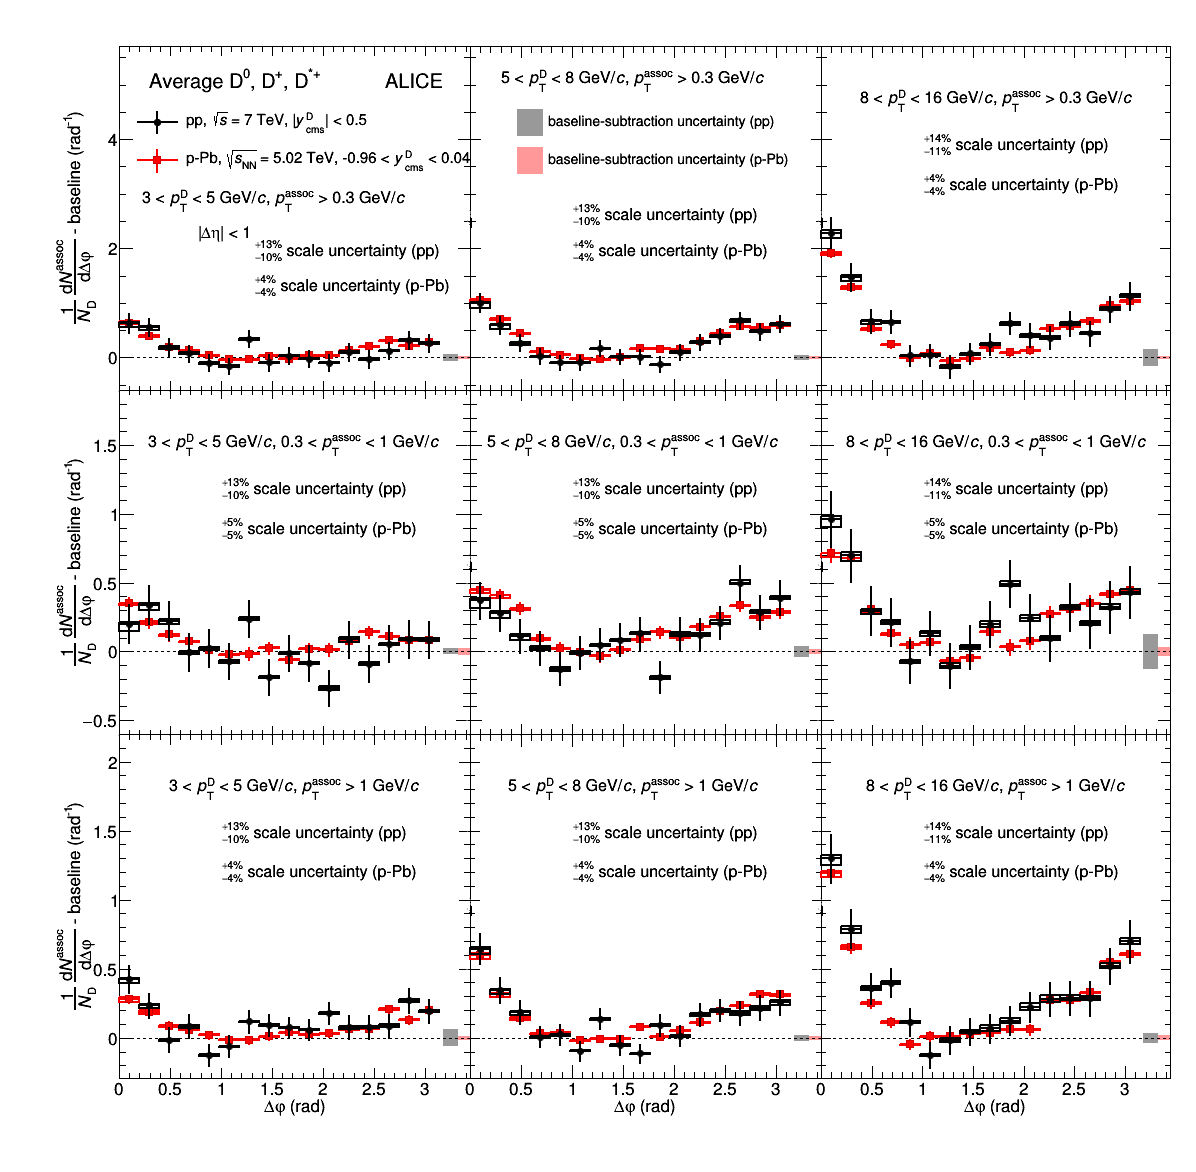
\includegraphics[width=\linewidth]{figures/CfrPPandModels/plotComparison_WeightedAverage_pp_pPb_UniqueCanvas_Style1.png}}
\caption{Comparison of pp 2010 (black) and p-Pb 2016 (red) average D-h azimuthal correlation distributions, for the common $\pt$ ranges.}
\label{fig:CfrppCorrel}
\end{figure}

In Figure \ref{fig:CfrppObs} the comparison is performed for the near-side peak observables, again in the common kinematic ranges, where the same consideration about the uncertainties holds. The similarity of the correlation distributions is reflected also in the near-side yield and width values, which do not seem to differ within the uncertainties, pointing to the absence of strong effects from cold-nuclear matter effects on the correlation distributions.

It has to be said that, on the base of a study performed with Pythia6-Perugia2011 simulations, a scaling factor of about 0.93 is expected when passing from a center-of-mass energy of $\rm{\sqrts = 7 ~ TeV}$ to $\rm{\sqrts = 5}$ TeV, difficult to be appreciated with the current uncertainties, especially the pp ones.

\begin{figure}[!htbp]
\centering
{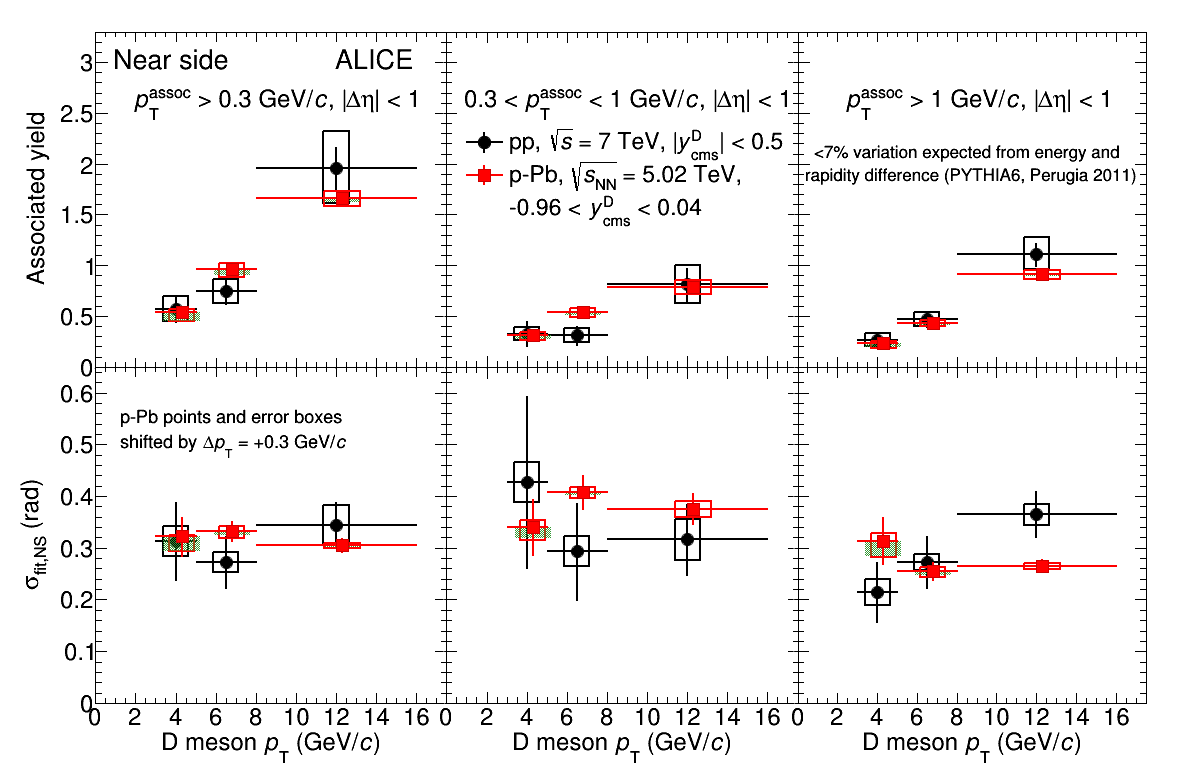
\includegraphics[width=\linewidth]{figures/CfrPPandModels/ComparePPtoPPbFitResults.png}}
\caption{Comparison of pp 2010 (black) and p-Pb 2016 (red) near-side peak yields and widths, for the common $\pt$ ranges.}
\label{fig:CfrppObs}
\end{figure}
